% Created by tikzDevice version 0.10.1 on 2017-11-28 18:58:33
% !TEX encoding = UTF-8 Unicode
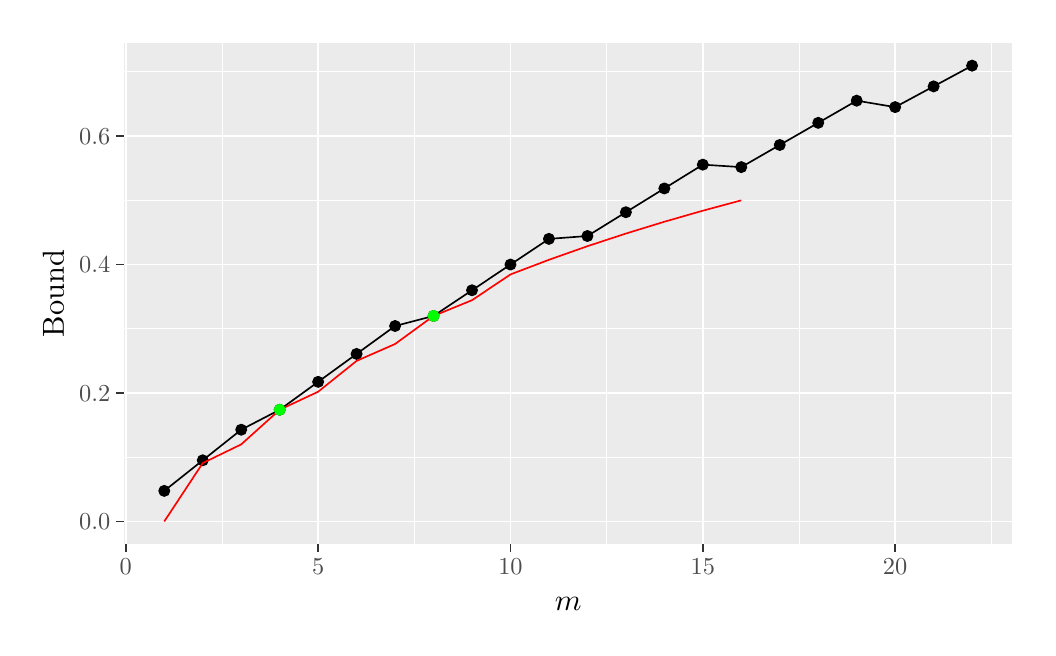
\begin{tikzpicture}[x=1pt,y=1pt]
\definecolor{fillColor}{RGB}{255,255,255}
\path[use as bounding box,fill=fillColor,fill opacity=0.00] (0,0) rectangle (361.35,216.81);
\begin{scope}
\path[clip] (  0.00,  0.00) rectangle (361.35,216.81);
\definecolor{drawColor}{RGB}{255,255,255}
\definecolor{fillColor}{RGB}{255,255,255}

\path[draw=drawColor,line width= 0.6pt,line join=round,line cap=round,fill=fillColor] (  0.00,  0.00) rectangle (361.35,216.81);
\end{scope}
\begin{scope}
\path[clip] ( 34.77, 30.14) rectangle (355.85,211.31);
\definecolor{fillColor}{gray}{0.92}

\path[fill=fillColor] ( 34.77, 30.14) rectangle (355.85,211.31);
\definecolor{drawColor}{RGB}{255,255,255}

\path[draw=drawColor,line width= 0.3pt,line join=round] ( 34.77, 61.58) --
	(355.85, 61.58);

\path[draw=drawColor,line width= 0.3pt,line join=round] ( 34.77,108.00) --
	(355.85,108.00);

\path[draw=drawColor,line width= 0.3pt,line join=round] ( 34.77,154.41) --
	(355.85,154.41);

\path[draw=drawColor,line width= 0.3pt,line join=round] ( 34.77,200.83) --
	(355.85,200.83);

\path[draw=drawColor,line width= 0.3pt,line join=round] ( 70.21, 30.14) --
	( 70.21,211.31);

\path[draw=drawColor,line width= 0.3pt,line join=round] (139.71, 30.14) --
	(139.71,211.31);

\path[draw=drawColor,line width= 0.3pt,line join=round] (209.21, 30.14) --
	(209.21,211.31);

\path[draw=drawColor,line width= 0.3pt,line join=round] (278.71, 30.14) --
	(278.71,211.31);

\path[draw=drawColor,line width= 0.3pt,line join=round] (348.21, 30.14) --
	(348.21,211.31);

\path[draw=drawColor,line width= 0.6pt,line join=round] ( 34.77, 38.38) --
	(355.85, 38.38);

\path[draw=drawColor,line width= 0.6pt,line join=round] ( 34.77, 84.79) --
	(355.85, 84.79);

\path[draw=drawColor,line width= 0.6pt,line join=round] ( 34.77,131.21) --
	(355.85,131.21);

\path[draw=drawColor,line width= 0.6pt,line join=round] ( 34.77,177.62) --
	(355.85,177.62);

\path[draw=drawColor,line width= 0.6pt,line join=round] ( 35.46, 30.14) --
	( 35.46,211.31);

\path[draw=drawColor,line width= 0.6pt,line join=round] (104.96, 30.14) --
	(104.96,211.31);

\path[draw=drawColor,line width= 0.6pt,line join=round] (174.46, 30.14) --
	(174.46,211.31);

\path[draw=drawColor,line width= 0.6pt,line join=round] (243.96, 30.14) --
	(243.96,211.31);

\path[draw=drawColor,line width= 0.6pt,line join=round] (313.46, 30.14) --
	(313.46,211.31);
\definecolor{drawColor}{RGB}{0,0,0}
\definecolor{fillColor}{RGB}{0,0,0}

\path[draw=drawColor,line width= 0.4pt,line join=round,line cap=round,fill=fillColor] ( 49.36, 49.43) circle (  1.96);

\path[draw=drawColor,line width= 0.4pt,line join=round,line cap=round,fill=fillColor] ( 63.26, 60.48) circle (  1.96);

\path[draw=drawColor,line width= 0.4pt,line join=round,line cap=round,fill=fillColor] ( 77.16, 71.53) circle (  1.96);

\path[draw=drawColor,line width= 0.4pt,line join=round,line cap=round,fill=fillColor] ( 91.06, 78.74) circle (  1.96);

\path[draw=drawColor,line width= 0.4pt,line join=round,line cap=round,fill=fillColor] (104.96, 88.83) circle (  1.96);

\path[draw=drawColor,line width= 0.4pt,line join=round,line cap=round,fill=fillColor] (118.86, 98.92) circle (  1.96);

\path[draw=drawColor,line width= 0.4pt,line join=round,line cap=round,fill=fillColor] (132.76,109.01) circle (  1.96);

\path[draw=drawColor,line width= 0.4pt,line join=round,line cap=round,fill=fillColor] (146.66,112.64) circle (  1.96);

\path[draw=drawColor,line width= 0.4pt,line join=round,line cap=round,fill=fillColor] (160.56,121.92) circle (  1.96);

\path[draw=drawColor,line width= 0.4pt,line join=round,line cap=round,fill=fillColor] (174.46,131.21) circle (  1.96);

\path[draw=drawColor,line width= 0.4pt,line join=round,line cap=round,fill=fillColor] (188.36,140.49) circle (  1.96);

\path[draw=drawColor,line width= 0.4pt,line join=round,line cap=round,fill=fillColor] (202.26,141.52) circle (  1.96);

\path[draw=drawColor,line width= 0.4pt,line join=round,line cap=round,fill=fillColor] (216.16,150.12) circle (  1.96);

\path[draw=drawColor,line width= 0.4pt,line join=round,line cap=round,fill=fillColor] (230.06,158.71) circle (  1.96);

\path[draw=drawColor,line width= 0.4pt,line join=round,line cap=round,fill=fillColor] (243.96,167.31) circle (  1.96);

\path[draw=drawColor,line width= 0.4pt,line join=round,line cap=round,fill=fillColor] (257.86,166.42) circle (  1.96);

\path[draw=drawColor,line width= 0.4pt,line join=round,line cap=round,fill=fillColor] (271.76,174.42) circle (  1.96);

\path[draw=drawColor,line width= 0.4pt,line join=round,line cap=round,fill=fillColor] (285.66,182.42) circle (  1.96);

\path[draw=drawColor,line width= 0.4pt,line join=round,line cap=round,fill=fillColor] (299.56,190.43) circle (  1.96);

\path[draw=drawColor,line width= 0.4pt,line join=round,line cap=round,fill=fillColor] (313.46,188.10) circle (  1.96);

\path[draw=drawColor,line width= 0.4pt,line join=round,line cap=round,fill=fillColor] (327.36,195.59) circle (  1.96);

\path[draw=drawColor,line width= 0.4pt,line join=round,line cap=round,fill=fillColor] (341.26,203.08) circle (  1.96);

\path[draw=drawColor,line width= 0.6pt,line join=round] ( 49.36, 49.43) --
	( 63.26, 60.48) --
	( 77.16, 71.53) --
	( 91.06, 78.74) --
	(104.96, 88.83) --
	(118.86, 98.92) --
	(132.76,109.01) --
	(146.66,112.64) --
	(160.56,121.92) --
	(174.46,131.21) --
	(188.36,140.49) --
	(202.26,141.52) --
	(216.16,150.12) --
	(230.06,158.71) --
	(243.96,167.31) --
	(257.86,166.42) --
	(271.76,174.42) --
	(285.66,182.42) --
	(299.56,190.43) --
	(313.46,188.10) --
	(327.36,195.59) --
	(341.26,203.08);
\definecolor{drawColor}{RGB}{255,0,0}

\path[draw=drawColor,line width= 0.6pt,line join=round] ( 49.36, 38.38) --
	( 63.26, 59.47) --
	( 77.16, 66.23) --
	( 91.06, 78.74) --
	(104.96, 85.26) --
	(118.86, 96.40) --
	(132.76,102.50) --
	(146.66,112.64) --
	(160.56,118.33) --
	(174.46,127.64) --
	(188.36,132.93) --
	(202.26,137.84) --
	(216.16,142.41) --
	(230.06,146.68) --
	(243.96,150.67) --
	(257.86,154.41);
\definecolor{drawColor}{RGB}{0,255,0}
\definecolor{fillColor}{RGB}{0,255,0}

\path[draw=drawColor,line width= 0.4pt,line join=round,line cap=round,fill=fillColor] ( 91.06, 78.74) circle (  1.96);

\path[draw=drawColor,line width= 0.4pt,line join=round,line cap=round,fill=fillColor] (146.66,112.64) circle (  1.96);
\end{scope}
\begin{scope}
\path[clip] (  0.00,  0.00) rectangle (361.35,216.81);
\definecolor{drawColor}{gray}{0.30}

\node[text=drawColor,anchor=base east,inner sep=0pt, outer sep=0pt, scale=  0.88] at ( 29.82, 35.35) {0.0};

\node[text=drawColor,anchor=base east,inner sep=0pt, outer sep=0pt, scale=  0.88] at ( 29.82, 81.76) {0.2};

\node[text=drawColor,anchor=base east,inner sep=0pt, outer sep=0pt, scale=  0.88] at ( 29.82,128.18) {0.4};

\node[text=drawColor,anchor=base east,inner sep=0pt, outer sep=0pt, scale=  0.88] at ( 29.82,174.59) {0.6};
\end{scope}
\begin{scope}
\path[clip] (  0.00,  0.00) rectangle (361.35,216.81);
\definecolor{drawColor}{gray}{0.20}

\path[draw=drawColor,line width= 0.6pt,line join=round] ( 32.02, 38.38) --
	( 34.77, 38.38);

\path[draw=drawColor,line width= 0.6pt,line join=round] ( 32.02, 84.79) --
	( 34.77, 84.79);

\path[draw=drawColor,line width= 0.6pt,line join=round] ( 32.02,131.21) --
	( 34.77,131.21);

\path[draw=drawColor,line width= 0.6pt,line join=round] ( 32.02,177.62) --
	( 34.77,177.62);
\end{scope}
\begin{scope}
\path[clip] (  0.00,  0.00) rectangle (361.35,216.81);
\definecolor{drawColor}{gray}{0.20}

\path[draw=drawColor,line width= 0.6pt,line join=round] ( 35.46, 27.39) --
	( 35.46, 30.14);

\path[draw=drawColor,line width= 0.6pt,line join=round] (104.96, 27.39) --
	(104.96, 30.14);

\path[draw=drawColor,line width= 0.6pt,line join=round] (174.46, 27.39) --
	(174.46, 30.14);

\path[draw=drawColor,line width= 0.6pt,line join=round] (243.96, 27.39) --
	(243.96, 30.14);

\path[draw=drawColor,line width= 0.6pt,line join=round] (313.46, 27.39) --
	(313.46, 30.14);
\end{scope}
\begin{scope}
\path[clip] (  0.00,  0.00) rectangle (361.35,216.81);
\definecolor{drawColor}{gray}{0.30}

\node[text=drawColor,anchor=base,inner sep=0pt, outer sep=0pt, scale=  0.88] at ( 35.46, 19.13) {0};

\node[text=drawColor,anchor=base,inner sep=0pt, outer sep=0pt, scale=  0.88] at (104.96, 19.13) {5};

\node[text=drawColor,anchor=base,inner sep=0pt, outer sep=0pt, scale=  0.88] at (174.46, 19.13) {10};

\node[text=drawColor,anchor=base,inner sep=0pt, outer sep=0pt, scale=  0.88] at (243.96, 19.13) {15};

\node[text=drawColor,anchor=base,inner sep=0pt, outer sep=0pt, scale=  0.88] at (313.46, 19.13) {20};
\end{scope}
\begin{scope}
\path[clip] (  0.00,  0.00) rectangle (361.35,216.81);
\definecolor{drawColor}{RGB}{0,0,0}

\node[text=drawColor,anchor=base,inner sep=0pt, outer sep=0pt, scale=  1.10] at (195.31,  6.06) {$m$};
\end{scope}
\begin{scope}
\path[clip] (  0.00,  0.00) rectangle (361.35,216.81);
\definecolor{drawColor}{RGB}{0,0,0}

\node[text=drawColor,rotate= 90.00,anchor=base,inner sep=0pt, outer sep=0pt, scale=  1.10] at ( 13.08,120.73) {Bound};
\end{scope}
\end{tikzpicture}
